\documentclass{article}
\usepackage[utf8]{inputenc}
\usepackage[margin=1in]{geometry}
\usepackage[utf8]{inputenc}
\usepackage{circuitikz}
\usepackage{hyperref}
\usepackage{braket} % supports quantum mechanical notation

\title{\texttt{circuitikz} Op Amp Examples}
\author{E.P. Blair}

\begin{document}


\maketitle

% ========================================
% ========================================
% ========================================
\section{Introduction}
% ========================================
% ========================================
% ========================================

In this \LaTeX ~document, I provide examples of circuit drawings.


% ========================================
% ========================================
% ========================================
\section{Ideal Op Amps}
% ========================================
% ========================================
% ========================================

Op amp circuits can be \textit{very} tricky to draw. Here are a few examples.

% ========================================
% ========================================
\subsection{Op amp only} 
% ========================================
% ========================================

Figure \ref{fig:basic_op_amp_only} provides an example of a circuit with an op amp, disconnected from any other circuit.

% ========================================
\begin{figure}[htbp]
    \centering
    \begin{circuitikz}[american]
    % Original circuit
    \draw
      (0, 0) node[op amp] (opamp) {}
      (opamp.-) to [short, -*] ++(-1, 0)
         [anchor=east] node  {$a$}
      (opamp.+) to [short, -*] ++(-1, 0)
         [anchor=east] node {$b$};
    \draw
      [very thick, ->] (-2.25, -0.825) node [anchor=north east] {$i_{+}$}
         to ++(0.75,0);
    \draw
      [very thick, ->] (-2.25, 0.825) node [anchor=south east]  {$i_{-}$}
         to ++(0.75,0);
    
    \end{circuitikz}
    \caption{Basic op amp.}
    \label{fig:basic_op_amp_only}
\end{figure}



% ========================================
% ========================================
\subsection{Buffer Op Amp} 
% ========================================
% ========================================

Figure \ref{fig:buffer} shows a basic buffer circuit.

% ========================================
\begin{figure}[htbp]
    \centering
    \begin{circuitikz}[american]
    % Op amp
    \draw
      (0, 0) node[op amp] (opamp) {}
      (opamp.-) to [short, -*] +(-1, 0)
         [anchor=north] node (a)  {$a$};
    \draw (opamp.+) to [short, -*] ++(-1, 0)
         [anchor=south] node (b) {$b$};

    % Voltage source
    %   Note: I have to start at (opamp.+) again to get the
    %         coordinates right. If i start at (b), it just
    %         looks off. I use [open] to avoid double-drawing
    %.        wires.
    \draw (opamp.+) to [open]  ++(-1, 0)
        to [short] ++(-2,0)
        to [V, l=$v_{in}$] ++(0,-2) node [ground] {};
        
    % Feedback path + output
    % This makes use of what I call "composite coordinates"
    %  Example: let (A) and (B) be saved as nodes/coordinates
    %       (A -| B) is the y-coord. of A, and x-coord. of B
    %       (A |- B) is the vertical (y) component of B, and the horizontal (x) component of A
    \draw (opamp.-) to [open] ++(-1, 0)
        to [short] ++(0,2) node (ref_x) {} % I'll reference this coordinate
        to [short] (opamp.out |- ref_x)
        to [short] (opamp.out)
        to [short, -*] ++(2,0)
        to [open, v=$v_{out}$] ++(0, -2)
        to [short, -] ++(0,-0.5) node [ground] {};
    % current arrows
    \draw [very thick, ->] (-2,-0.75)
        to ++(0.75,0) [anchor=north east] node {$i_{in}$};
    \draw [very thick, ->] (-2,0.75)
        to ++(0.75,0) [anchor=south east] node {$i_{-}$};
    \end{circuitikz}
    \caption{This circuit is a basic buffer circuit. No feedback or input resistance is included. \label{fig:buffer}}
\end{figure}
% ========================================


% ========================================
% ========================================
\subsection{Non-inverting Op Amp} 
% ========================================
% ========================================

Figure \ref{fig:non-inv-op-amp} shows a basic inverting op amp circuit.

% ========================================
\begin{figure}[htbp]
    \centering
    \begin{circuitikz}[american]
    % Original circuit
    \draw
      (0, 0) node[op amp] (opamp) {}
      (opamp.-) to [short, -*] +(-1, 0)
         [anchor=north] node (a)  {$a$};
    % draw node b
    \draw (opamp.+) to [short, -*] ++(-1, 0)
         [anchor=south] node (b) {$b$};

    \draw (opamp.-) to [open] ++(-1, 0) % open (circuit) avoids double-drawing 
         to [R, l=$R_1$] ++(-4,0)
         to [short] ++(0,-2.75) node (gnd) [ground] {};
    \draw (opamp.+) to [open] ++(-1,0)
         to [short] ++(-1,0) node (alpha) {}
         to [V, l_=$v_{\mbox{in}}$] (alpha|-gnd)
         to [short] (gnd);
    \draw (opamp.out) to [short, -*] ++(1,0)
         to [open, v_=$v_{\mbox{out}}$] ++(0, -2)
         to [short, *-] ++(0,-0.5) node [ground] {};
    % This makes use of what I call "composite coordinates"
    %  Example: let (A) and (B) be saved as nodes/coordinates
    %       (A -| B) is the vertical component of A, and the horizontal component of B
    %       (A |- B) is the vertical component of B, and the horizontal component of A
    \draw (a)  % node a and feedback path
        to [short] ++(0,2) node (R2left) {} % "save" left side of R2 as (R2left)
        to [R, l=$R_2$] (R2left -| opamp.out)
           node (R2right) {}  % "save" right side of R2 as (R2right)
        to [short] (opamp.out);
    % Current arrow
    \draw
      [very thick, ->] (-2, -0.825) node [anchor=north west] {$i_{+}$}
         to ++(0.5,0);
    \draw
      [very thick, ->] (-2, 0.825) node [anchor=south west]  {$i_{-}$}
         to ++(0.5,0);
     
      % (opamp.-) to [short,*-] ++(0,1.5) coordinate (leftC)
      % to[C] (leftC -| opamp.out)
      % to[short,-*] (opamp.out)    
    \end{circuitikz}
    \caption{Non-inverting op amp.}
    \label{fig:non-inv-op-amp}
\end{figure}
% ========================================


% ========================================
\subsection{Inverting op amp}
% ========================================

To make an inverting op amp, you can use the same techniques as before. If you wish to swap the inverting and non-inverting terminals, you can use the \texttt{yscale=-1} optional argument for the op amp (\href{https://tex.stackexchange.com/questions/49428/how-can-i-invert-the-poles-of-an-op-amp-in-circuitikz}{StackExchange thread link}).


% ========================================
% ========================================
% ========================================
\section{Quantum Circuits}
% ========================================
% ========================================
% ========================================

This is a system I worked out to draw quantum circuits before I learned about the \href{http://mirrors.ibiblio.org/CTAN/graphics/pgf/contrib/quantikz/quantikz.pdf}{\texttt{quantikz}} package. A basic circuit is shown in Figure \ref{fig:basic_quantum_circuit}.

\begin{figure}
    \centering
    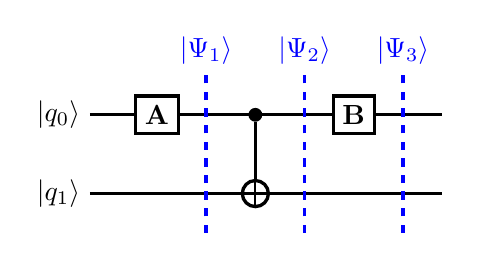
\begin{tikzpicture}
    % Create some reusable tikz styles
    \tikzset{
    cross/.style={path picture={ 
    \draw[thick,black](path picture bounding box.north) -- (path picture bounding box.south) (path picture bounding box.west) -- (path picture bounding box.east);
    }},
    circlewc/.style={draw, very thick, fill = white, circle,cross,minimum width=0.3 cm},
    }

    \tikzstyle{dot} = [fill,shape=circle,minimum size=5pt,inner sep=0pt]
    \tikzstyle{oplus} = [draw, very thick, fill=white,shape=circle,minimum size=10pt,inner sep=0pt]

    % x and y spacing units for circuit
    \newcommand{\dy}{1}
    \newcommand{\dx}{1.25}
    \newcommand{\cktwidth}{4*\dx}
    
    % q0 line
    % format: \node (x, y) (name) {string};
    \node at (0,0) (q0) {$\ket{q_0}$};
    \node (q0end) at (\cktwidth,0) {};
    \draw [very thick, -] (q0) -- (q0end);
    
    % q1 line
    \node at (0,-\dy) (q1) {$\ket{q_1}$};
    \node (q1end) at (\cktwidth,-\dy) {};
    \draw [very thick, -] (q1) -- (q1end);
    
    % Column 1
    \node (A01) [draw, very thick, fill=white] at (\dx, 0*\dy ) {$\mathbf{A}$};
    % \node (X11) [draw, very thick, fill=white] % at (\dx, -1*\dy ) {$\mathbf{X}$};
    
    % column 2
    \node[dot] (d02) at (2*\dx, 0*\dy) {};
    \node[circlewc] (c12) at (2*\dx, -1*\dy) {};
    \draw[very thick, .-] (c12) -- (d02);
    
    % column 3
    \node (B03) [draw, very thick, fill=white] at (3*\dx, 0*\dy ) {$\mathbf{B}$};
    
    \draw [color=blue, very thick, dashed, -] (1.5*\dx, -1.5*\dy)
        -- ++ (0, 2*\dy) node [anchor=south] {$\ket{\Psi_1}$};
    \draw [color=blue, very thick, dashed, -] (2.5*\dx, -1.5*\dy)
        -- ++ (0, 2*\dy) node [anchor=south] {$\ket{\Psi_2}$};
    \draw [color=blue, very thick, dashed, -] (3.5*\dx, -1.5*\dy)
        -- ++ (0, 2*\dy) node [anchor=south] {$\ket{\Psi_3}$};

\end{tikzpicture}
    \caption{This is a basic quantum circuit.}
    \label{fig:basic_quantum_circuit}
\end{figure}
\end{document}
